\section{Основные понятие}

\subsection{Вычисление булевой функции с помощью КНФ}
Рассмотрим булеву функцию $f(x_1, \dotsc, x_n) \colon \{0,1\}^n \to \{0,1\}$. 
Будем говорить, что КНФ~$F(x_1, \dotsc, x_n)$ \emph{вычисляет~$f$}, если $f \equiv F$, то есть, для всех $x_1, \dotsc, x_n \in \{0,1\}$, $f(x_1, \dotsc, x_n)=F(x_1, \dotsc, x_n)$. 
Будем представлять КНФ как множество клозов, и под размером КНФ будем подразумевать количество клозов. Известно, что для любой функции $f$ существует КНФ, вычисляющая ее. 
Один из способов построить такую КНФ следующий: для каждого входа $x \in \{0,1\}^n$, такого что $f(x) = 0$ добавим в КНФ клоз длины $n$, который опровергает $x$.

Этот метод не гарантирует, что полученная КНФ будет иметь минимальное число клозов:
было бы слишком хорошо, будь это иначе, 
ведь задача поиска КНФ минимального размера для данной булевой функции $f$ (заданной с помощью таблицы истинности) является NP-трудной, как доказал~Масек~\cite{MasekNpComp} 
(смотри также \cite{DBLP:journals/siamcomp/AllenderHMPS08} и ссылки там).
Например, для функции  $f(x_1,x_2)=x_1$ этот метод
создает КНФ $(\overline{x_1} \lor x_2) \land (\overline{x_1} \lor \overline{x_2})$, хотя функция $x_1$ уже представлена в виде КНФ.

\subsection{Функция четности}
Известно, что для многих функций минимальный размер КНФ, вычисляющей их, экспоненциальный. 
Каноническим примером такой функции является четность: $\PAR_n(x_1, \dotsc, x_n)=x_1 \oplus \dotsb \oplus x_n$. 
Основное свойство этой функции, из - за которого она не может быть посчитана короткой КНФ,~---~это высокая \emph{чувствительность}:
если в любом входе поменять значение любого бита на противоположенный,
то значение всей функции изменится на противоположенное.

\begin{lemma}\label{lemma:detparity}
	Минимальный размер КНФ, вычисляющей~$\PAR_n$ имеет размер $2^{n-1}$
\end{lemma}
\begin{proof}
	Верхняя границы следует из метода, описанного выше и того факта, что $|\PAR_n^{-1}(0)|=2^{n-1}$.
	
	Нижняя оценка основана на том, что любой клоз в КНФ $f$, вычисляющей $\PAR_n$ должен содержать все переменные $x_1, \dotsc, x_n$ или их отрицания. 
	Предположим, что это не так.
	Пусть есть клоз $C \in F$, который не зависит от $x_i$ (то есть $x_i \not \in C$ и $\overline{x_i} \not \in C$).
	Рассмотрим вход $x \in \{0, 1\}^n$, который не удовлетворяет $C$, 
	тогда $F(x)=\PAR_n(x)=0$. 
	Но если в этом входе поменять значение $x_i$ на противоположенное, 
	то клоз $C$ будет все еще не удовлетворен. 
	Противоречие с высокой чувствительностью функции четности. 
	Таким образом, все клозы $F$ имеют ровно $n$ переменных (или их отрицаний), 
	а значит каждый клоз может опровергнуть ровно одно значение
	 $x \in \{0, 1\}^n$. 
	Но опровергающих значений у $\PAR_n$ $2^{n-1}$, значит должно быть хотя бы $2^{n - 1}$ клозов.
	
\end{proof}

\subsection{Кодировка булевой функции с помощью КНФ}
Будем говорить, что КНФ $F$ \emph{кодирует} булеву функцию $f(x_1, \dotsc, x_n)$, если выполняются следующие два условия:
\begin{enumerate}
	\item В дополнение ко входным битам $x_1, \dotsc, x_n$, $F$~также зависит от  $s$~ битов $y_1, \dotsc, y_s$, называемые \emph{дополнительным} или \emph{недетерминированным входом}.
	\item Для любых $x \in \{0,1\}^n$, $f(x)=1$ если и только если существует $y \in \{0,1\}^s$ такой, что $F(x,y)=1$. Другими словами, для всех $x \in \{0,1\}^n$,
	\begin{equation}\label{eq:enc}
		f(x) = \bigvee_{y \in \{0,1\}^s}F(x,y) \, .
	\end{equation}
\end{enumerate}
Такое представление булевой функции широко используется на практике при переводе задач на язык КНФ. Например, так выглядит одна из КНФ-кодировок функции $\PAR_4$: 
\begin{multline}\label{eq:toyenc}
	(x_1 \lor x_2 \lor \overline{y_1}) \land (x_1 \lor  \overline{x_2} \lor y_1) \land (\overline{x_1} \lor x_2 \lor y_1) \land (\overline{x_1} \lor \overline{x_2} \lor \overline{y_1})
	\land
	(y_1 \lor x_3 \lor \overline{y_2}) \land\\ (y_1 \lor  \overline{x_3} \lor y_2) \land (\overline{y_1} \lor x_3 \lor y_2) \land (\overline{y_1} \lor \overline{x_3} \lor \overline{y_2})
	\land (\overline{x_4} \lor y_2) \land (x_4 \lor \overline{y_2}) \, .
\end{multline}
\subsection{Булева схема и преобразование Цейтина}
Одним из естественных способом получения КНФ-кодировки булевой функции $f$ является преобразование Цейтина~\cite{zbMATH03325539}. 
А именно, надо взять булеву схему, вычисляющую $f$, и применим к ней преобразование Цейтина. 
Наглядно продемонстрируем это на игрушечном примере. 
Рассмотрим схему, вычисляющую функцию $\PAR_{12}$, которая приведена ниже. 
Она имеет $12$~входов, $3$~гейта (один из которых выходной)
и ее глубина равна трем.

\tikzstyle{gate} = [circle, draw, inner sep=0mm, minimum size=5mm]

\begin{center}
	\begin{tikzpicture}[yscale=1]
		%\draw[help lines] (1,0) grid (12,3);
		\begin{scope}[xscale=0.7, yscale=0.7]
			\foreach \n in {1,...,12}
			\node (\n) at (\n,0) {$x_{\n}$};
			\foreach \x/\y/\n/\l/\edges in {2.5/1/y1/y_1/{1,2,3,4}, 6.5/1.5/y2/y_2/{5,6,7,8,y1}, 10.5/2/y_3/y_3/{9,10,11,12,y2}} {
				\node[gate,label=above:$\l$] (\n) at (\x,\y) {$\oplus$};
				\foreach \i in \edges
				\draw[->] (\i) -- (\n);
			}
		\end{scope}
		\node[right, text width=42mm, inner sep=0mm] at (9,.75) {
			$y_1=x_1 \oplus x_2 \oplus x_3 \oplus x_4$\\
			$y_2=y_1 \oplus x_5 \oplus x_6 \oplus x_7 \oplus x_8$\\
			$y_3=y_2 \oplus x_9 \oplus x_{10} \oplus x_{11} \oplus x_{12}$
		};
	\end{tikzpicture}
\end{center}

Справа от схемы приведены функции, вычисляемые каждым гейтом. 
Преобразуем каждое равенство в КНФ, соберем все КНФ в одну и добавим в нее клоз  $(y_3)$. 
Полученная КНФ кодирует функцию, которую вычисляет схема. 
Отметим, что КНФ~\eqref{eq:blocks} получена таким же способом
(после распространения значения выходного гейта).

КНФ может быть представлена в виде схемы глубины $2$,
в которой выходной гейт будет вычислять $AND$, все остальные гейты~---~$OR$, 
и входы~---~это переменные или их отрицания.
Например, следующая схема соответствует КНФ~\eqref{eq:toyenc}. 
Такие схемы глубины $2$ также обозначаются, как  $\AND \circ \OR$  схемы. 

\begin{center}
	\begin{tikzpicture}[xscale=.9, yscale=.5, >=latex]
		%\draw[help lines] (0,0) grid (14,5);
		
		\foreach \n\s in {1/x_1, 2/x_2, 3/\overline{y_1},
			4/x_1, 5/\overline{x_2}, 6/y_1,
			7/\overline{x_1}, 8/x_2, 9/y_1,
			10/\overline{x_1}, 11/\overline{x_2}, 12/\overline{y_1},
			13/y_1, 14/x_3, 15/\overline{y_2},
			16/y_1, 17/\overline{x_3}, 18/y_2,
			19/\overline{y_1}, 20/x_3, 21/y_2,
			22/\overline{y_1}, 23/\overline{x_3}, 24/\overline{y_2}}
		\node (v_\n) at (0.5 * \n - 0.5, 0) {$\s$};
		
		\node (v_25) at (12.3, 0) {$y_2$};
		\node (v_26) at (12.7, 0) {$\overline{x_4}$};
		\node (v_27) at (13.7, 0) {$\overline{y_2}$};
		\node (v_28) at (14.3, 0) {$x_4$};
		
		\foreach \m in {1,...,10}
		\node[gate] (y\m) at (-1 + 1.5 * \m, 2) {$\lor$};
		
		\foreach \n in {2,...,25} {
			\def\qq{\the\numexpr\n / 3}
			\def\tt{\the\numexpr\qq}
			\def\dec{\the\numexpr\n - 1}
			\draw[->] (v_\dec) -- (y\tt);
		}
		
		\draw[->] (v_25) -- (y9);
		\draw[->] (v_26) -- (y9);
		\draw[->] (v_27) -- (y10);
		\draw[->] (v_28) -- (y10);
		
		\node[gate] (z) at (7.25, 4.5) {$\land$};
		
		\foreach \n in {1,...,10}
		\draw[->] (y\n) -- (z);
		
	\end{tikzpicture}
\end{center}

\subsection{Схемы глубины 3}
Естественным обобщением конъюнктивной нормальной формы являются схемы глубины $3$: 
~\emph{$\Sigma_3$-схема}~---~это OR нескольких КНФ.
В схеме клозы могут быть общие у разных КНФ. 
\emph{$\Sigma_3$-формула}~---~это $\Sigma_3$-схема, КНФы которой не имеют общих клозов 
(другими словами, это схема, у которой выходная степень каждого гейта не больше $1$).
 
С одной стороны, это вычислительная модель все еще достаточно простая. 
С другой стороны, доказать нижние оценки в такой модель оказывается трудно:
получить нижнюю оценку $2^{\omega(n)}$ на размер явной функции (скажем, из $NP$ или $E^{NP}$) это серьезная задача.
Получение нижней оценки $2^{\omega(n/\log \log n)}$ разрешит еще один открытый вопрос за счет уменьшения глубины Вейлинта~\cite{DBLP:conf/mfcs/Valiant77}: 
доказательство суперлинейной нижней оценки на размер схем логарифмической глубины.
Подробнее об известные результатах со схемами глубины $3$ есть в книге Юкны~\cite[Chapter~11]{DBLP:books/daglib/0028687}.
Для функции четности лучшая известная нижняя оценка на схему глубины $3$~---~это ~$\Omega(2^{\sqrt{n}})$~\cite{DBLP:journals/cjtcs/PaturiPZ99}, 
на формулу глубины $3$~---~это $\Omega(2^{2\sqrt{n}})$~\cite{DBLP:journals/eccc/Hirahara17}. 
Обе нижние оценки оптимальны с точностью до полиномиального фактора.

Равенство~\eqref{eq:enc} показывает тесную связь между КНФ-кодировками и схемами глубины $3$ типа  $\OR \circ \AND \circ \OR$. В самом деле, пусть \\ $F(x_1, \dotsc, x_n, y_1, \dotsc, y_s)=\{C_1, \dotsc, C_m\}$~---~это КНФ-кодировка булевой функции $f \colon \{0,1\}^n \to \{0,1\}$.
Тогда $f(x)=\lor_{y \in \{0,1\}^s}F(x,y)$.
Перебрав все возможные $2^n$ означиваний для $y$-ов, можно получить $\Sigma_3$ формулу, вычисляющую $f$:
\begin{equation}\label{eq:expansion}
	f(x)=\bigvee_{j \in [2^s]}F_j(x) \, ,
\end{equation}
где каждая $F_j$ является КНФ.
Будем называть это~\emph{расширением} $F$.
Например, расширение КНФ~\eqref{eq:toyenc} выглядит следующим образом. Это OR четырех КНФ.

\begin{center}
	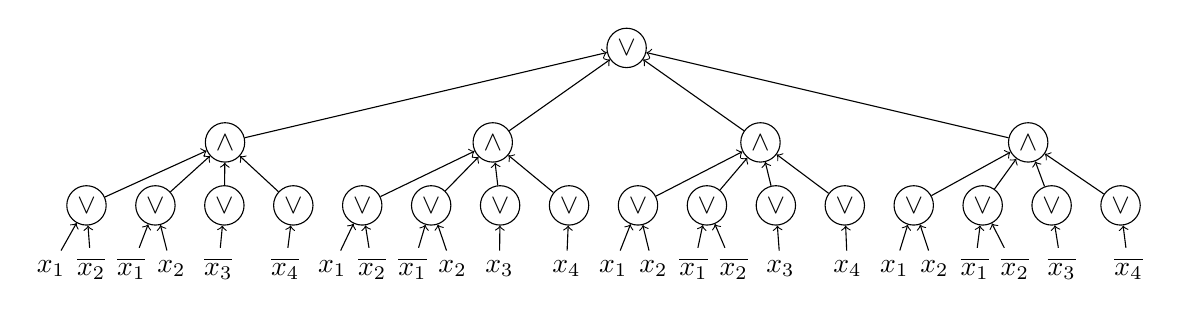
\begin{tikzpicture}[xscale=.85, yscale=.4]
		%\draw[help lines] (0,0) grid (15,7);
		
		\foreach \n\s\dx\t in {1/x_1/-1.1/0, 2/\overline{x_2}/-0.5/0, 3/\overline{x_1}/-0.9/1,
			4/x_2/-0.3/1, 5/\overline{x_3}/-0.6/2, 6/\overline{x_4}/-0.6/3,
			7/x_1/-0.9/4, 8/\overline{x_2}/-0.3/4, 9/\overline{x_1}/-0.7/5,
			10/x_2/-0.1/5, 11/x_3/-0.4/6, 12/x_4/-0.4/7,
			13/x_1/-0.7/8, 14/x_2/-0.1/8, 15/\overline{x_1}/-0.5/9,
			16/\overline{x_2}/0.1/9, 17/x_3/-0.2/10, 18/x_4/-0.2/11,
			19/x_1/-0.5/12, 20/x_2/0.1/12, 21/\overline{x_1}/-0.3/13,
			22/\overline{x_2}/0.3/13, 23/\overline{x_3}/0/14, 24/\overline{x_4}/0/15
		}
		\node (v_\n) at (\t+\dx, 0) {$\s$};
		
		\foreach \m in {1,...,16}
		\node[circle, draw, inner sep=0mm, minimum size=5mm] (y\m) at (-1.6 + 1.03 * \m, 2) {$\lor$};
		
		\foreach \m in {1,...,4}
		\node[circle, draw, inner sep=0mm, minimum size=5mm] (z\m) at (-2.5 + 4 * \m, 4) {$\land$};
		
		\node[circle, draw, inner sep=0mm, minimum size=5mm] (q) at (7.5, 7) {$\lor$};
		
		\foreach \n in {1,...,4}
		\draw[->] (z\n) -- (q);
		
		\foreach \n\m in {1/1, 2/1, 3/1, 4/1, 5/2, 6/2, 7/2, 8/2,
			9/3, 10/3, 11/3, 12/3, 13/4, 14/4, 15/4, 16/4}
		\draw[->]  (y\n) -- (z\m);
		
		\foreach \n\m in {1/1, 2/1, 3/2, 4/2, 5/3, 6/4,
			7/5, 8/5, 9/6, 10/6, 11/7, 12/8,
			13/9, 14/9, 15/10, 16/10, 17/11, 18/12,
			19/13, 20/13, 21/14, 22/14, 23/15, 24/16}
		\draw[->] (v_\n) -- (y\m);
	\end{tikzpicture}
\end{center}
Расширение~---~это формула, это OR нескольких КНФ, каждый гейт имеет выходную степень не больше $1$. 
Аналогичном способом можно получить \emph{расширение схемы}: 
в этом случае гейтам разрешено иметь выходную степень больше $1$, 
то есть КНФы могут иметь общие клозы. 
Например, это расширение схемы все того же примера~\eqref{eq:toyenc}.

\begin{center}
	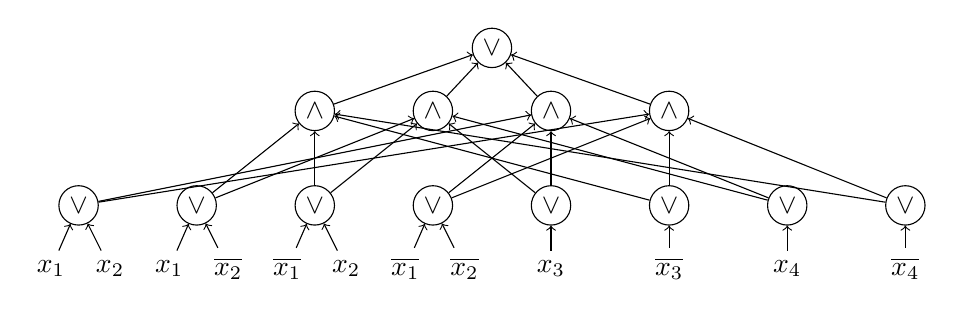
\begin{tikzpicture}[yscale=.4]
		%\draw[help lines] (0,0) grid (11,7);
		
		\foreach \n\s in {1/x_1, 2/x_2,
			3/x_1, 4/\overline{x_2},
			5/\overline{x_1}, 6/x_2,
			7/\overline{x_1}, 8/\overline{x_2}}
		\node (v_\n) at (0.75 * \n-0.6, 0) {$\s$};
		\foreach \n\s in {9/x_3, 10/\overline{x_3},
			11/x_4, 12/\overline{x_4}}
		\node (v_\n) at (1.5 * \n-7, 0) {$\s$};
		
		\foreach \m in {1,...,8}
		\node[circle, draw, inner sep=0mm, minimum size=5mm] (y\m) at (-1 + 1.5 * \m, 2) {$\lor$};
		
		\foreach \m in {1,...,4}
		\node[circle, draw, inner sep=0mm, minimum size=5mm] (z\m) at (2 + 1.5 * \m, 5) {$\land$};
		
		\node[circle, draw, inner sep=0mm, minimum size=5mm] (q) at (5.75, 7) {$\lor$};
		
		\foreach \n in {1,...,4}
		\draw[->] (z\n) -- (q);
		
		\foreach \n\m in {1/3, 1/4, 2/1, 2/2, 3/1, 3/2, 4/3, 4/4,
			5/2, 5/3, 6/1, 6/4, 7/2, 7/3, 8/1, 8/4}
		\draw[->]  (y\n) -- (z\m);
		
		\foreach \n\m in {1/1, 2/1, 3/2, 4/2, 5/3, 6/3, 7/4, 8/4,
			9/5, 10/6, 11/7, 12/8}
		\draw[->] (v_\n) -- (y\m);
		
	\end{tikzpicture}
\end{center}

Ниже будет показано, что КНФ-кодировка и схема глубины $3$ могут быть легко преобразованы друг в друга.
Для удобства, определим размер схемы как число гейтов \emph{исключая} выходной.
В таком случае, размер КНФ формулы равен числу клозов (КНФ~---~это схема глубины $2$).
Под~$\Sigma_3(t,r)$-схемой будем обозначать $\Sigma_3$-схему 
имеющую не более~$t$~AND-ов на втором слое и не более~$r$~OR-ов на третьем слое (то есть ее размер не больше $t + r$). 

\begin{lemma}
	Пусть $F(x_1, \dotsc, x_n, y_1, \dotsc, y_s)$~---~это КНФ-кодировка размера~$m$ функции
	$f \colon \{0,1\}^n \to \{0,1\}$.
	Тогда, $f$~может быть посчитана
	с помощью $\Sigma_3(2^s, m \cdot 2^s)$-формулы
	и с помощью $\Sigma_3(2^s,m)$-схемы.
\end{lemma}
\begin{proof}
	Пусть $F=\{C_1, \dotsc, C_m\}$. Чтобы расширить $F$ как $\bigvee_{j \in [2^s]}F_j$,
	мы переберем все $2^s$ означивание дополнительных переменных
	$y_1, \dotsc, y_s$. В каждом таком означивании каждый клоз $C_i$
	либо становится выполненным, либо превращается в клоз $C_i' \subseteq C_i$
	($C_i'$~---~это клоз $C_i$, в котором удалили все дополнительные переменные).
	Таким образом, для каждого $j \in [2^s]$, $F_j \subseteq \{C_1', \dotsc, C_m'\}$.
	Соответствующая $\Sigma_3$-формула содержит не более $2^s+m2^s$ гейтов:
	есть $2^s$ гейтов для $F_j$, каждая $F_j$ содержит не более, чем $m$~клозов.
	Соответствующая $\Sigma_3$-схема содержит не более, чем $2^s+m$ гейтов:
	есть $2^s$ гейтов для $F_j$ и $m$~гейтов для $C_1', \dotsc, C_m'$
	(каждая $F_j$ выбирает какие из этих $m$~клозов содержать).
\end{proof}

Стоит отметить, что нижняя граница на схемы глубины $3$, полученная с помощью такого преобразования не может быть существенно улучшена.
Действительно, взяв КНФ-кодировку функции $\PAR_n$ c $s = \sqrt{n}$ и $m = O(\sqrt{n}2^{\sqrt{n}})$ (как в \eqref{eq:blocks}), 
можно получить $\Sigma_3$-формулу и $\Sigma_3$-схему размера $2^{2\sqrt{n}}$ и $2^{\sqrt{n}}$ соответственно, с точностью до полиномиального фактора. 
Как уже было сказано выше, известно, что эти оценки оптимальны (с обеих сторон).

Ниже мы покажем обратное преобразование.

\begin{lemma}\label{lemma:circuit2encoding}
	Пусть $C$~---~это $\Sigma_3(t,r)$-формула (схема), вычисляющая булеву функцию $f \colon \{0,1\}^n \to \{0,1\}$. Тогда можно получить КНФ-кодировку $f$ с~$\lceil \log t \rceil$ дополнительными переменными и размера $r$ ($2rt$, соответственно).
\end{lemma}
\begin{proof}
	Пусть $C=F_1 \lor \dotsb \lor F_{t}$ - это $\Sigma_3$-формула (тогда, $r=\size(F_1)+\dotsb+\size(F_{t})$). Введем $s=\lceil\log t\rceil$ дополнительных переменных $y_1, \dotsc, y_s$. Теперь для каждого означивания $y_1, \dotsc, y_s$, возьмем соответствующую КНФ $F_i$ ($1 \le i \le 2^s$ - однозначное целочисленное соответствие 
	этому означиванию) и добавим
	$y_i$ с соответствующим знаком в каждый клоз $F_i$.
	Назовем получившуюся КНФ $F_i'$. Тогда, $F=F_1'\land \dotsb \land F_{2^s}'$ кодирует $f$ и $F$ имеет не больше $r$~клозов.
	
	Если $C$ это $\Sigma_3$-схема, то создадим отдельные копии каждого гейта, соответствующего клозам каждой из $2^s$ КНФ. 
	Таким образом, размер получившейся КНФ-кодировки не больше, чем  $r2^s \le 2rt$.
\end{proof}

В заключение, покажем, что доказать сильные нижние оценки на размер КНФ-кодировки -
не проще, чем доказать сильные нижние оценки на размер формул глубины $3$.
Пусть $C$~---~это $\Sigma_3(t,r)$-формула, вычисляющая $\PAR_n$.
Лемма~\ref{lemma:circuit2encoding} гарантирует, что $\PAR_n$ может быть закодирована как КНФ размера $r$ с $\lceil \log t \rceil$ дополнительными переменными. 
Тогда, согласно неравенству\eqref{eq:sm},
\[\size(C) = t + r \ge t + \Omega \left( \frac{1}{n}\cdot 2^{\frac{n}{\log t + 2}} \right) \ge \frac 1n \left( t + \Omega\left( 2^{\frac{n}{\log t + 2}}\right)\right) \ge \Omega\left(\frac{2^{\sqrt{n}}}{n}\right) \, .\]
Аналогично, если $C$~---~это $\Sigma_3(t,r)$-схема. Лемма~\ref{lemma:circuit2encoding} гарантирует, что $\PAR_n$ может быть закодирована как КНФ размера $2rt$ с $\lceil \log t \rceil$ дополнительными переменными.
Тогда,
\[\size(C) = t + r \ge t + \Omega \left( \frac{1}{2tn}\cdot 2^{\frac{n}{\log t + 2}} \right) \ge \Omega\left(\frac{2^{\sqrt{n/2}}}{n}\right) \, .\]